\section{Grådige algoritmer}
En grådig algoritme er en algoritme som velger den beste lokale løsningen. Det vi si at den velger en lokalt optimal løsning i håp om at den også skal være globalt optimal.
\\\\
Problemene vi bruker grådighetsalgoritmer på ligner ofte veldig på problemene som er beskrevet tidligere i dette kapittelet. Vi har fortsatt optimal substruktur og vi har valg. Forskjellen ligger i at valgene er mye enklere. Vi tviler ikke lenger på hva som er best, en ting skiller seg klart ut og vi kan velge det hver gang uten å trenge å vurdere de andre. Merk at det ikke alltid vil fungere å bruke en grådig algoritme.
\\\\
Problemer som kan løses med grådige algoritmer har ikke nødvendigvis overlappende delproblemer, men de har det som kalles \textit{greedy-choice property}. Det går ut på at et valg som er lokalt optimalt (dvs. at det ser ut som et godt valg her og nå) er den del av den globalt optimale løsningen (dvs. at det vil føre frem å ta det grådige valget).

\subsection{Huffmankode}
Huffmankode er en særdeles effektiv teknikk for å komprimere data. Ideen er å ha en variabel lengde på kodebitene. For eksempel i en enkel tekstfil lar man de bokstavene som forekommer ofte ha en kort kode, og de man bruker sjelden gir man en lang kode.
\\\\
En prefikskode er slik at intet kodeord også er et prefiks til et annet kodeord. Dette gjør dem meget lett å dekode, for man trenger da ikke vite hvor et ord slutter og et annet begynner. En dekodingsprosess trenger en hendig representasjon for prefiks-koden slik at det opprinnelige kodeordet lett blir funnet. En god representasjon er rett og slett et binærtre hva bladene er de gitte bokstavene. Huffman fant opp en grådighetsalgoritme som konstruerer en optimal prefikskode. Huffman-algoritmen bruker frekvensen til de forskjellige bokstavene og lager et binærtre.

\begin{boxed}
Anta at vi sender noe informasjon som kun innehar bokstavene e, r, s og t. Vi vet også den relative frekvensen til bokstavene. Dette er vist i tabellen:
\begin{table}[H]
    %\caption{}
    \label{tab:huffman1}
    \centering
    \begin{tabular}{|L{5em} |L{5em}|L{5em}|L{5em}|L{5em}|}
        \hline
        \rowcolor[HTML]{303F9F}
        \textbf{\textcolor{white}{Bokstav}} & \textbf{\textcolor{white}{e}} & \textbf{\textcolor{white}{r}} & \textbf{\textcolor{white}{s}} & \textbf{\textcolor{white}{t}}\\
        \rowcolor[HTML]{E6E6E6}
        Frekvens & 45 & 27 & 15 & 13\\
         \hline
    \end{tabular}
\end{table}
Nå bruker vi algoritmen til Huffman steg for steg og kommer til slutt fram til det optimale binærtreet for disse fore bokstavene. Dermed har vi koden til de forskjellige bokstavene, som blir:
\begin{table}[H]
    %\caption{}
    \label{tab:huffman1}
    \centering
    \begin{tabular}{|L{5em} |L{5em}|L{5em}|L{5em}|L{5em}|}
        \hline
        \rowcolor[HTML]{303F9F}
        \textbf{\textcolor{white}{Bokstav}} & \textbf{\textcolor{white}{e}} & \textbf{\textcolor{white}{r}} & \textbf{\textcolor{white}{s}} & \textbf{\textcolor{white}{t}}\\
        \rowcolor[HTML]{E6E6E6}
        Kode & 0 & 10 & 111 & 110\\
         \hline
    \end{tabular}
\end{table}
Legg merke til at dette er en prefikskode. Ordet ''se'' blir 1110, ordet ''erterester'' blir da 0101100100111110010.

\begin{figure}[H]
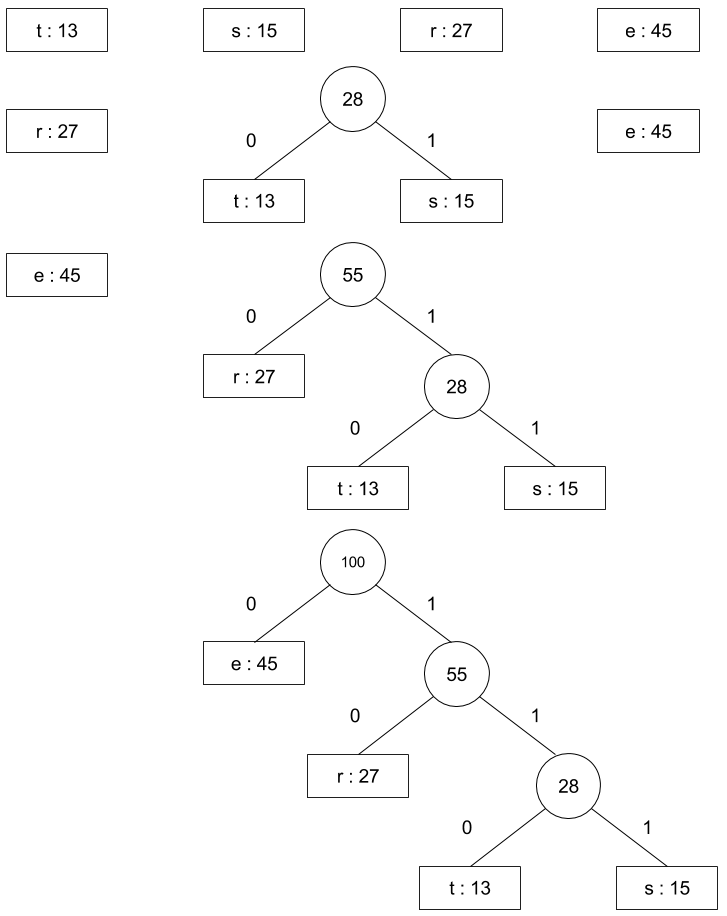
\includegraphics[scale=0.47]{images/huffman}
\centering %centering the image
\caption{Huffman-tre}
\label{fig:huffman}
\end{figure}
\end{boxed}